\documentclass[11pt]{beamer}
\usepackage{listings} 
\usepackage[T1]{fontenc}
\usepackage[utf8]{inputenc}
\usepackage[english]{babel}
\usepackage{amsmath}
\usepackage{amssymb, amsfonts, latexsym, cancel}
\usepackage{float}
\usepackage{graphicx}
\usepackage{epstopdf}
\usepackage{subfigure}
\usepackage{hyperref}
%\usepackage{authblk}
\usepackage{blindtext}
\usepackage{booktabs}
\usepackage{filecontents}
\usepackage{courier}
\usepackage{listings}
\lstset{
tabsize = 2, 
showstringspaces = false 
numbers = left, 
commentstyle = \color{green}
keywordstyle = \color{blue}
stringstyle = \color{red} 
rulecolor = \color{black}
basicstyle = \small \ttfamily 
breaklines = true
numberstyle = \tiny,
}
\usepackage{caption}
\DeclareCaptionFont{white}{\color{white}}
\DeclareCaptionFormat{listing}{\colorbox{gray}{\parbox{\textwidth}{#1#2#3}}}
\captionsetup[lstlisting]{format=listing,labelfont=white,textfont=white}
\definecolor{urlColor}{rgb}{0.0, 0.0, 204}
\definecolor{linkColor}{rgb}{0.57, 0.0, 0.04}
\definecolor{fileColor}{rgb}{0.0, 0.26, 0.26}
\definecolor{textoColor}{rgb}{0, 0, 240}
\hypersetup{
    colorlinks=true,
    linkcolor=linkColor,
    filecolor=fileColor,      
    urlcolor=urlColor,
}
\urlstyle{same}
\setbeamercovered{transparent}
%\usetheme{Boadilla}
\usetheme{CambridgeUS}
%\usetheme{Berkeley}
%\usetheme{Warsaw}
%\usetheme{Madrid}

\title[principles]{\bf\Huge EARLY POO}
\subtitle{class and package design}
\author[ pcontreras y  dfloressi]
{Contreras Huamani, Paul Michaell\\ Flores Silva, David }
\institute[UNSA]
{\inst{1}% 
System Engineering School\\
System Engineering and Informatic Department\\
Production and Services Faculty\\
San Agustin National University of Arequipa
}
\date[2020-04-01]{\scriptsize{2020-04-01}}


\begin{document}
\titlepage

\begin{frame}
\frametitle{Content}
\tableofcontents
\end{frame}

\section{Class design}
\begin{frame}
\frametitle{ Class design}
\framesubtitle{symptoms of a class design}
\begin {itemize}
\item Rigidity.
\item Fragidity.
\item Inmovility.
\item Viscosity.
\item Innesesary Complexity.
\item Innesesary Repetition.
\item Opacity.
\end{itemize}
\end{frame}


\begin{frame}
\textbf{1.- Rigidity}\\
\textcolor{urlColor}{classes are difficult to change}\\
\textbf{2.- Fragidity}\\
\textcolor{urlColor}{classes stop working}\\
\textbf{3.- Inmovility}\\
\textcolor{urlColor}{classes are difficult to reuse}\\
\textbf{4.- Viscosity}\\
\textcolor{urlColor}{classes are difficult to use}\\
\textbf{5.- Innesesary Complexity}\\
\textcolor{urlColor}{overdesigned}\\
\textbf{6.- Innesesary Repetition}\\
\textcolor{urlColor}{copy and paste}\\
\textbf{7.- Opacity}\\
\textcolor{urlColor}{messy}\\
\end{frame}

\section{principles of class designs}
\begin{frame}
\frametitle{Principles of class designs}
\framesubtitle{Eliminate the symptoms of a Class Design}
\begin {itemize}
\item Sole responsability.
\item Open and closed.
\item Liskov substitution.
\item Independence investment.
\item Interface segregation.
\end{itemize}
\end{frame}

\begin{frame}
\textbf{1.- Sole responsability}\\
\textcolor{textoColor}{only reason to change}\\
\textbf{2.- Open and closed}\\
\textcolor{urlColor}{open extended and closed modify}\\
\textbf{3.- Liskov subtitution}\\
\textcolor{urlColor}{
is replaced by subtypes...}\\
\textbf{4.- Independence investment}\\
\textcolor{urlColor}{details depend on abstractions}\\
\textbf{5.- Interface segregation}\\
\textcolor{urlColor}{
a class does not depend on interfaces that do not use}\\
\end{frame}


\begin{frame}
\textbf{\begin{center}
\textcolor{textoColor}{BASIC EXAMPLE}
\end{center}}
\begin{center}
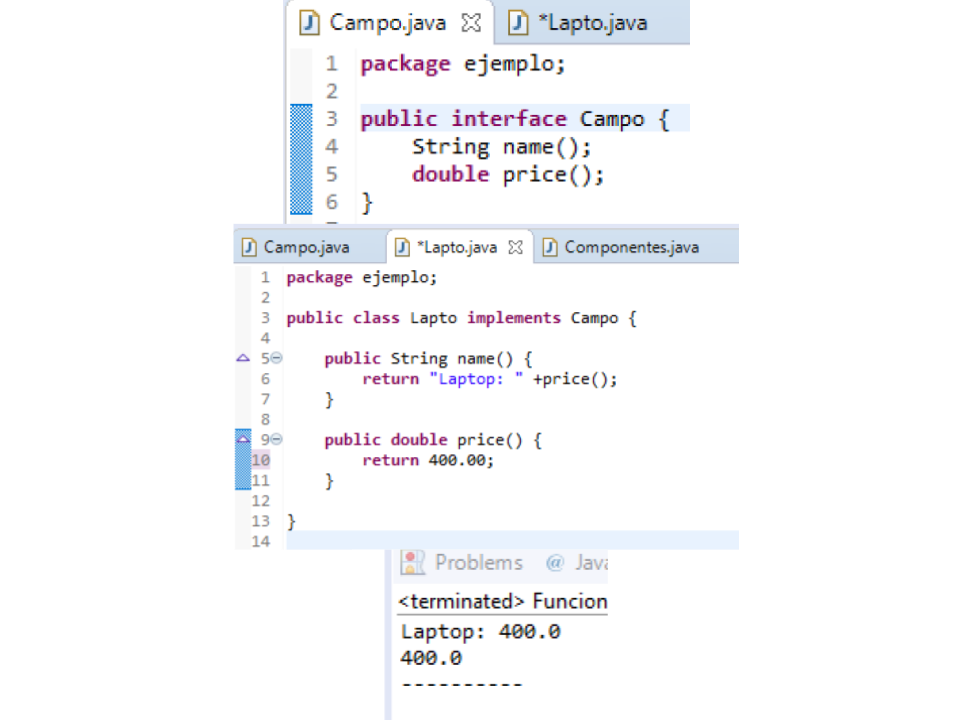
\includegraphics[scale=0.3]{D:/DAVID/PROGRAMAS DE Ing. SIST/LaTex/practicas de LaTex/planilla/img/ejemplo basico.png} 
\end{center}
\end{frame}

\begin{frame}
\textbf{\begin{center}
\textcolor{textoColor}{ADVANCED EXAMPLE}
\end{center}}
\begin{center}
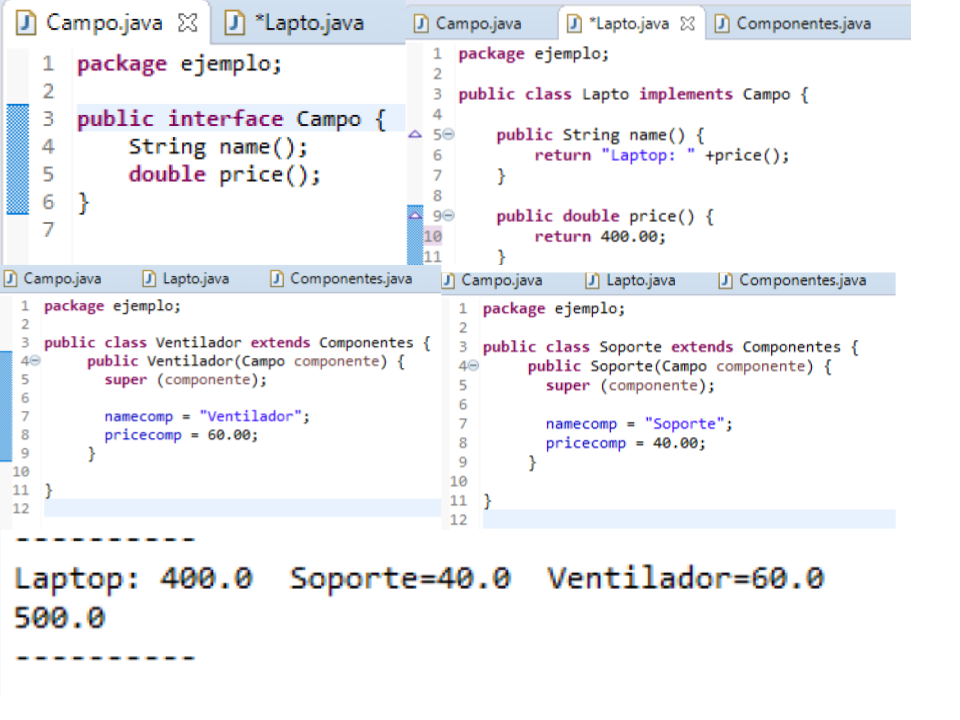
\includegraphics[scale=0.3]{D:/DAVID/PROGRAMAS DE Ing. SIST/LaTex/practicas de LaTex/planilla/img/ejemplo avanzado.png} 
\end{center}
\end{frame}

\begin{frame}
\begin{center}
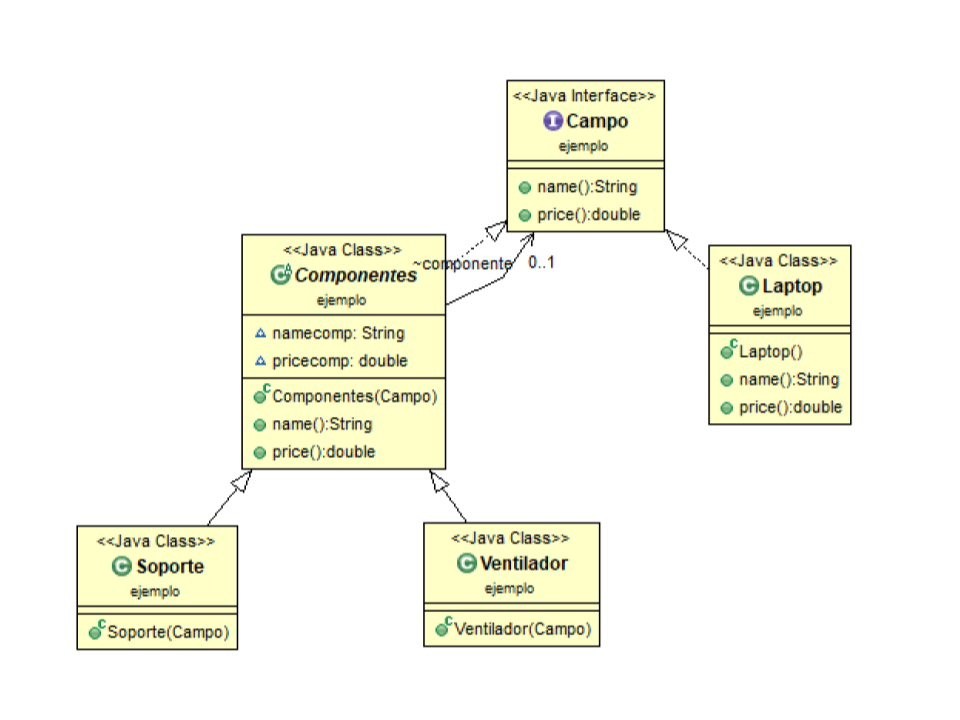
\includegraphics[scale=0.3]{D:/DAVID/PROGRAMAS DE Ing. SIST/LaTex/practicas de LaTex/planilla/img/clases.png} 
\end{center}
\end{frame}

\section{classes abstract and interface}
\begin{frame}
\frametitle{Classes abstract and interface}
An abstract class has two main functions which are:\\
\begin {itemize}
  \item has no instance.
  \item subclasses are defined.
\end {itemize}  
And an interface is declared with the keyword \textbf{INTERFACE} and it works
\begin {itemize}
  \item method statements.
  \item cannot instantiate.
  \item appear on packages.
\end {itemize}

\end{frame}

\section{Package design}
\begin{frame}
\frametitle{Package design}
\framesubtitle{Cohesion and coupling}
\begin {itemize}
\item Granularity: The cohesion of the packages
\item Stability: The coupling between packages

\end{itemize}
\end{frame}

\section{Case study: Mobile phone network}
\begin{frame}
\frametitle{Case study: Mobile phone network}
\framesubtitle{Operation of a mobile telephone network}
 Elements : \\
 \begin{center}
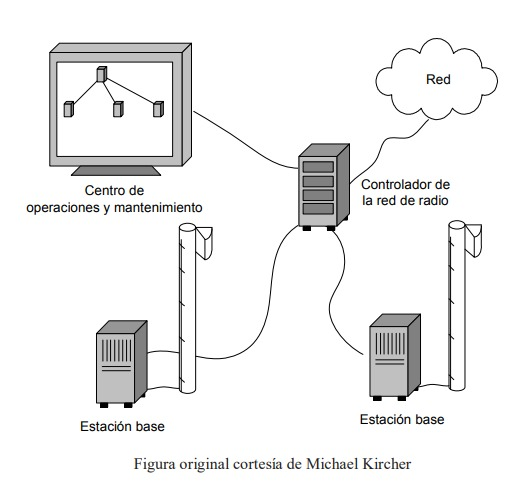
\includegraphics[scale=0.4]{D:/DAVID/PROGRAMAS DE Ing. SIST/LaTex/practicas de LaTex/planilla/img/elementos.jpg} 
\end{center}
\end{frame}

\begin{frame}
\frametitle{The architecture of a base station}
\textbf{1.- Base station hardware}\\
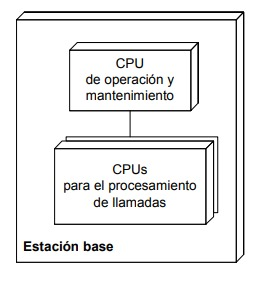
\includegraphics[scale=0.5]{D:/DAVID/PROGRAMAS DE Ing. SIST/LaTex/practicas de LaTex/planilla/img/Base Station Hardware.jpg}  
\end{frame}
\begin{frame}
\textbf{2.- Base station software}\\
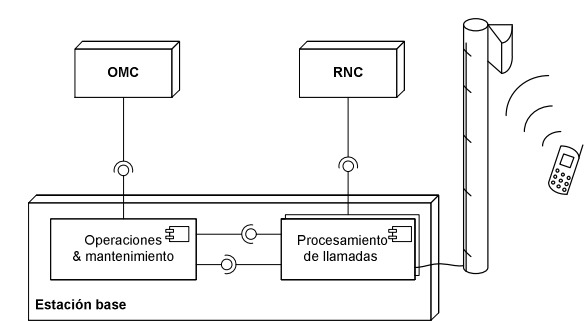
\includegraphics[scale=0.5]{D:/DAVID/PROGRAMAS DE Ing. SIST/LaTex/practicas de LaTex/planilla/img/Base Station Software.jpg} 
\end{frame}

\begin{frame}
\frametitle{OMC software architecture}
\textbf{1.- Functions of OMC}\\
\begin {itemize}
\item Communication with base stations and RNCs.
\item Discovery of base stations.
\item Maintaining network status.
\item Configuration of network elements.
\item Base Station Software Update.
\end{itemize} 


\textbf{2.- OMC software architecture}\\
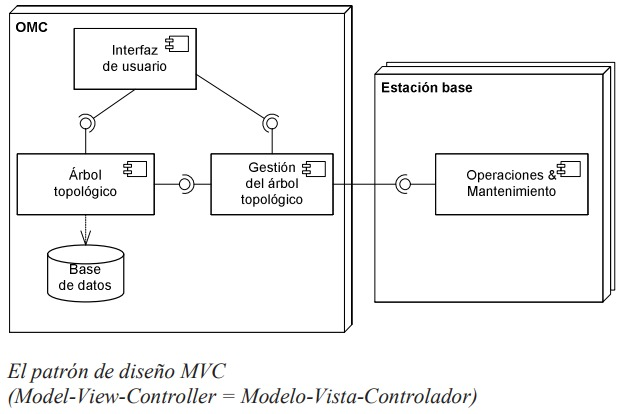
\includegraphics[scale=0.3]{D:/DAVID/PROGRAMAS DE Ing. SIST/LaTex/practicas de LaTex/planilla/img/OMC arquitectura software.jpg} 
\end{frame}
\textbf{3.- The OMC software is organized according to the MVC pattern}\\
\begin {itemize}
\item Model.\\
\item view.\\
\item Controller.\\
\end{itemize} 

\begin{frame}
\textbf{\begin{center}
\textcolor{textoColor}{BASIC EXAMPLE 2}\\
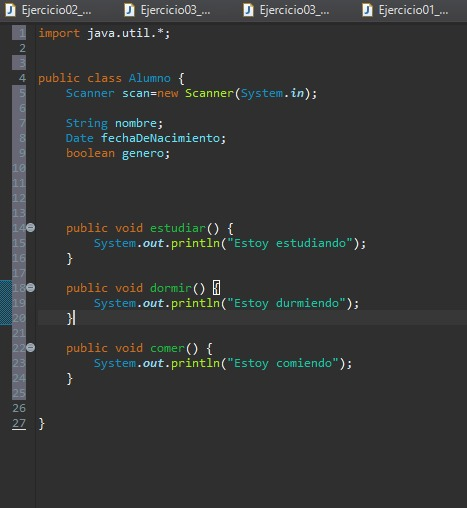
\includegraphics[scale=0.3]{../planilla/img/basic example2.jpg} 
\end{center}}
\end{frame}

\begin{frame}
\textbf{\begin{center}
\textcolor{textoColor}{ADVANCED EXAMPLE 2}\\
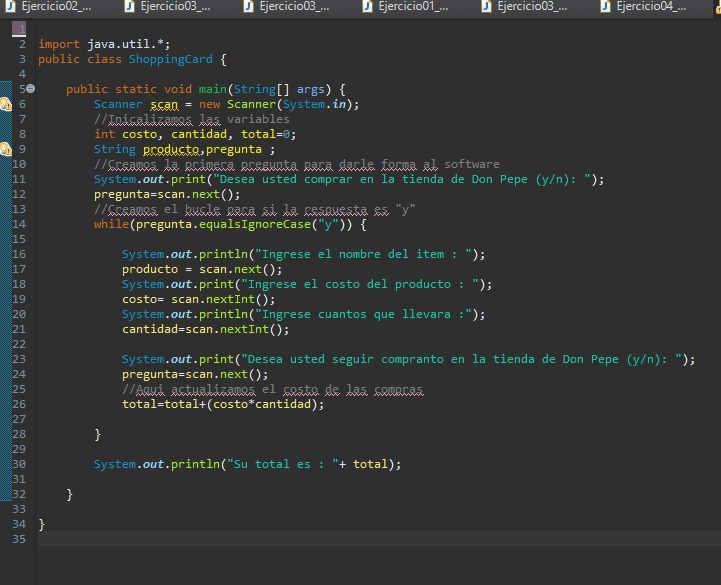
\includegraphics[scale=0.3]{../planilla/img/ejemplo avanzado2.jpg} 
\end{center}}
\end{frame}


\section{bibliography}
\begin{frame}
BIBLIOGRAPHY

1. https://elvex.ugr.es/decsai/java/\\
2. https://www.instintoprogramador.com.mx/2020/07/principio-abierto-cerrado.html\\
3. https://desarrolloweb.com/articulos/principio-sustitucion-liskov-dotnet.html\\
4. https://elvex.ugr.es/decsai/java/pdf/AB-classes.pdf\\
5. https://elvex.ugr.es/decsai/java/pdf/AD-packages.pdf\\
6. https://elvex.ugr.es/decsai/java/pdf/AF-ejercicios.pdf\\
\end{frame}
\end{document}

